
\begin{table}
	\caption{Dataset Statistics for CHEMET}
	\centering
	\begin{tabular}{lllll}
		
		\toprule
		Setting &Anno.& \#Inst. & \#Mention  & \#Types \\
		\midrule
		Train &Distant&   8000& NA&43\\
		Dev &Human&1000&NA&NA\\
		Test&Human&            1000&NA&NA \\
		\bottomrule
	\end{tabular}
	\label{datastats}
\end{table}



\begin{figure*}[ht]
% 	\vskip 0.2in
	\begin{center}
		\centerline{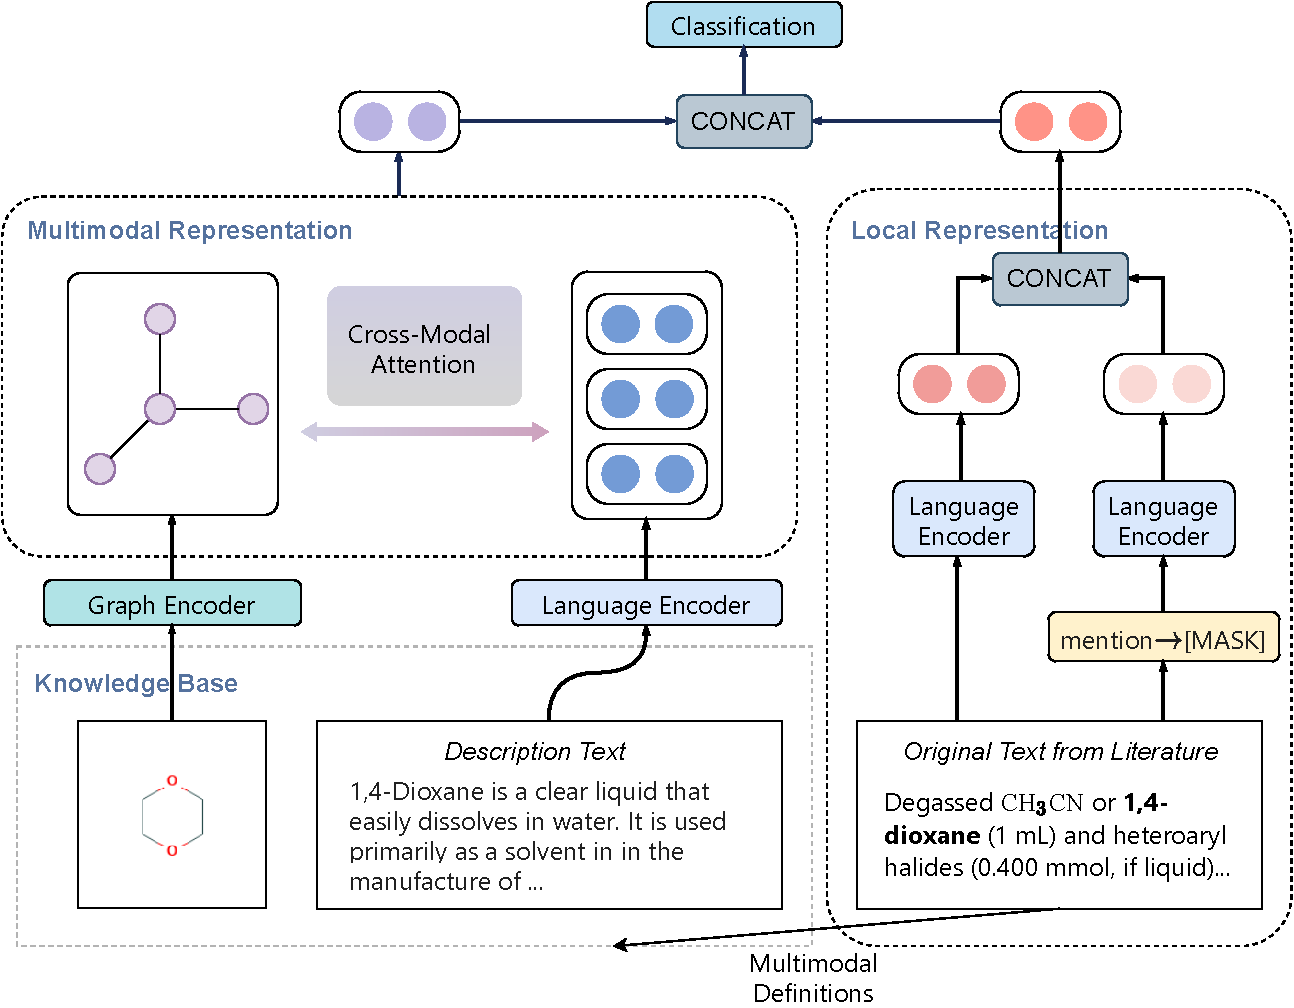
\includegraphics[width=2
			\columnwidth]{model_new.pdf}}
		\caption{Our fine-grained chemical entity typing model architecture. Please refer to Section~\ref{sec:method} for details. \heng{1. label "KB" and "Literature"; 2. make font bigger. }
		}
		\label{fig:framework}
	\end{center}
	\vskip -0.2in
\end{figure*}
\section{Dataset}
%\subsection{Data Collection}
\label{datacollection}

% Krippendorff alpha, or other 
% agreement metric

% describe diversity

\cheng{"limited dataset" is a bit vague. Is there any such data set available? If so, we should try to use it. My sense is that there isn't(?), so the novelty and significance of the data set could be more clearly articulated.}
\bluetext{Since there is no dataset available for fined-grained chemical entity typing, we have collected and annotated a dataset, CHEMET, based on a corpus of 100 papers from PubChem) with Suzuki-Coupling (a popular reaction mechanism) theme; the theme was chosen to align with chemistry annotators' domain knowledge. We will discuss the steps taken to construct the dataset below.}

\noindent \textbf{Taxonomy Construction}. \cheng{how was the number xx determined? try to give a justification or explanation of the process that reached the number xx. }\bluetext{In taxonomy construction, we focus on collecting the types that belong to chemicals commonly occurring in Suzuki-Coupling literature. We carefully select sub-categories from wikipedia chemistry category page~\footnote{\url{https://en.wikipedia.org/wiki/Category:Chemistry}} as fine-grained ontology; for example, Organic chemistry$\rightarrow$Organic compounds$\rightarrow$Esters is a fined-grained type where right of the arrow is the sub-category of the left. The ontology is shown in Appendix~\ref{sec:appendix1}}
% \cheng{The following sentence can be moved earlier in this paragraph to explain the strategy being taken. It's better to first give a description of our goal/strategy/philosophy and then describe how we do it. If there are decisions to be made, explain why we've decided to choose one options not another.} 

\noindent \textbf{Distant Supervision} 

% In order to ease human annotators' work and to collect training data, we employed distant supervision to retrieve noisy labels for the corpus. In this step we first tokenized text using~\cite{oscar4}, a texting mining framework for chemistry that recognize complex chemical name well. We then collected a dictionary mapping from picked types (that is, the select categories from Wikipedia) to their belonging wikipedia pages. We treated the page titles as entity names. Since a compound can have many synonyms, we queried PubChem to expand the dictionary. Finally, we used the dictionary to label the tokenized text using a well-performing string matching algorithm.
\cheng{Provide a reference to this string matching algorithm or elaborate.}

\jinfeng{I'm re-writing this section as below. Free free to use any part of it.}

We employed distant supervision from Wikipedia and PubChem to create noisy entity labels for the corpus. This process involves the following steps. 1) We first populated entities into the nodes (i.e., entity types) of the taxonomy. That generated an \textit{entity dictionary}. More details are given in the next paragraph. 2) We then tokenized the corpus using~\cite{oscar4}, a texting mining framework for chemistry that recognizes complex chemical name well. 3) Finally, we distantly labeled the corpus with the entity dictionary by following the procedure of training data generation in AutoNER \cite{DBLP:conf/emnlp/ShangLGRR018}.

Now we give more detailed description of our process of automatically assigning entities to types. Each type (except those starting with ``Other'') is a node in our taxonomy that corresponds to a category in Wikipedia. Each category can have sub-categories and associated pages. Starting from each type, we traced its sub-categories recursively by performing a depth-first search (DFS) with a maximum depth of three. In the DFS we skipped those sub-categories that are probably irrelevant to Chemistry. We used a spell-checker dictionary \cite{azman2012chemistry} with over 104,000 technical chemistry terms, and dropped a category from the search if less than 20\% of the 1-grams in its name and the names of all its direct children were covered by the dictionary. The maximum depth of three and threshold of 20\% were selected empirically by manually checking the quality of the results for some types. After the DFS, we populated the Wikipedia page titles associated with any sub-category of a type as entities of that type. For each type starting with ``Other'', we took the difference between the entities assigned to its direct parent category and those assigned to all its siblings as its entity list. Finally, we expanded each entity with its synonyms from the PubChem database\footnote{https://ftp.ncbi.nlm.nih.gov/pubchem/Compound/Extras/CID-Synonym-filtered.gz}.

\noindent \textbf{Human Annotation}.
Note: talk about agreement metric

% Note: talk about diversity

We hired five undergraduate chemistry students as annotators. The annotators were instructed to identify and type spans in the assigned samples using Brat~\cite{brat} interface. To ensure the diversity of the testing data, we randomly select the test samples from the corpus for annotation. In order to mitigate annotator bias, we distributed each sentence to three annotators, and take majority vote from the results. The dataset statistics is shown in Table~\ref{datastats}.


%\subsection{Data Analysis}

%\label{dataanalyze}
%\noindent \textbf{Size}. 
%
%\noindent \textbf{Entity Types}. 